\subsection{Modelo V3S}

V3S é um modelo com a finalidade de gerar ambientes para desenvolver treinamentos complexos em ambiente de realidade virtual visando atividades de risco e de emergência. O modelo é composto por três submodelos; \textit{Domain Model}, \textit{Activity Model} e \textit{Risk Model} \cite{v3sframework}. O \textit{Domain Model} é o núcleo do sistema. Todos os objetos, ações e relações são descritos por uma ontologia. 
A figura \ref{domainmodel} exibe a estrutura de classe desta ontologia.

\begin{figure}[H]
  \centering
  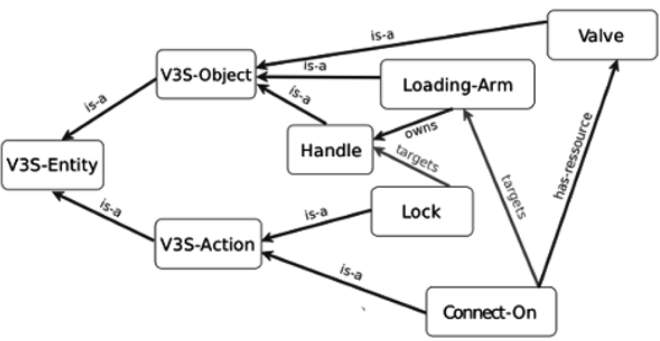
\includegraphics[width=0.5\linewidth]{figure/ontologyv3.png} 
  \caption{Ontologia que descreve \textit{Domain Model} no modelo V3S \cite{v3sframework}}
  \label{domainmodel}
\end{figure}

